\documentclass[a4paper, 12pt]{article}

%\usepackage{config}

% page margin 
\usepackage[
top=2cm,
right=2.5cm,
bottom=2cm,
left=2.5cm
]{geometry}

% language and characters
\usepackage[utf8]{inputenc}
\usepackage[T1]{fontenc}
\usepackage[brazilian]{babel}
\usepackage{indentfirst	}
\usepackage{
	amsmath,
	amsfonts,
	amssymb
}

% colors
\usepackage{xcolor}
\usepackage{float}

% watermark config
\usepackage{xwatermark}
%\newwatermark[allpages, scale=4, angle=60, color=red!30]{text}

% equations numbering
\numberwithin{equation}{section}

% graphics insertion
\usepackage{graphicx}
\usepackage{subfig}

% references in the document (for equations, sections, images, websites)
\usepackage{hyperref}
\usepackage[]{cleveref}

\usepackage{siunitx}

% manual draw
\usepackage{tikz}

\begin{document}
	\begin{titlepage}
		\begin{center}
			\textbf{\href{https://www.unicamp.br/unicamp/}{Universidade Estadual de Campinas}}\\\vspace{1cm}
			\href{https://www.feagri.unicamp.br/portal/}{Faculdade de Engenharia Agrícola}\\\vspace{5cm}
			%\textbf{}\\\vspace{1cm}
			\large{Trabalho Final de FA622}\\\vspace{4cm}
		\end{center}
		
		\hspace{8cm}\parbox{7cm}{Relatório apresentado como parte da avaliação da disciplina FA622 - Sistema Solo-Planta-Atmosfera, sob responsabilidade do Prof. Dr. José Teixeira}\\\vspace{4cm}
		
		RENAN DA SILVA GUEDES - 223979\\\vspace{4cm}
		\begin{center}
			CAMPINAS - SP\\\vspace{.2cm}
			AGOSTO
		\end{center}
		
	\end{titlepage}

	\newpage
	
	\tableofcontents
	\listoffigures
	
	\newpage
	
	\section{Introdução}

	A seguir temos um estudo referente às características de transpiração apresentadas pelas folhas de diferentes espécies vegetais. Com base nos gráficos, é possível analisar a transpiração foliar (E), o déficit de pressão de vapor (DPV) e a radiação fotossinteticamente ativa (PAR). Com bases nesses parâmetros foi possível obter os dados em diferentes instantes de tempo e potenciais hídricos das plantas ($\Psi_{\textrm{pd}}$) como é visto na legenda.

	\subsection{Cana de açúcar}	
	A primeira parte do estudo diz respeito à cana de açúcar variedade RB67515. Para a mesma a coleta de dados foi feita em duas datas, sendo a primeira em 17/08/2015 e a segunda em 19/10/2015 (Figuras 1 e 2). Com base nisso, nota-se que as duas coletas objetivaram a aquisição de dados em duas condições ambientais diferentes, permitindo comparar a variação dos parâmetros referidos com base em tal mudança.
	
	Quando analisamos a transpiração das plantas de cana nota-se que na primeira data -- 17/08/15 -- a taxa de transpiração foi menor em média quando comparado ao dia 19/10/15. Isso demonstra que a planta com maior potencial hídrico ($\Psi_{\textrm{pd}}=\SI{-0.14}{\mega\pascal}$) obteve a maior taxa de transpiração ($\textrm{E}$ por volta de $\SI{8.5}{\milli\mole\cdot\meter^{2}\cdot\second^{-1}}$). Entretanto, ao analisar o intervalo entre as 10h00 e 14h00 vê-se que a região onde ocorreu estabilização da taxa estava ao potencial de \SI{-.16}{\mega\pascal}, no dia 19/10/15, correspondendo a $\SI{2.85}{\milli\mole\cdot\meter^{2}\cdot\second^{-1}}$ de E. Quando é feita a mesma análise para o dia 17 temos que para $\Psi_{\textrm{pd}}=\SI{-0.18}{\mega\pascal}$ o valor de E foi de $\SI{2.56}{\milli\mole\cdot\meter^{2}\cdot\second^{-1}}$, demonstrando que a redução do $\Psi_{\textrm{pd}}$ é proporcional ao valor de E. 
	
	No que diz respeito à radiação fotossinteticamente ativa (PAR), vê-se que no dia 19 as médias dos valores de PAR para diferentes indivíduos são bem próximas, colaborando para o padrão de curvas sobrepostas observado. Todavia, para o dia 17 ao potencial de \SI{-18}{\mega\pascal} houve menor tendência de sobreposição. Nota-se que o maior valor de PAR ocorre para menores valores de potencial -- dia 17, correspondendo a $\SI{2010.50}{\micro\mole\cdot\meter^{-2}\cdot\second^{-1}}$ às 13h00.
	
	\subsection{Pata de vaca}
	Para a espécie pata de vaca, chegou-se que sob diferentes potenciais hídricos o maior valor de transpiração ocorreu entre as 12h00 e 14h00 em 28/11/16 correspondendo a $\SI{15.4}{\milli\mole\cdot\meter^{2}\cdot\second^{-1}}$. Em contrapartida, ao meio dia desta data a menor respiração ocorreu para o menor potencial $\Psi_{\textrm{pd}}=\SI{-0.13}{\mega\pascal}$. Isso demonstra que nos momentos onde há maior incidência de luz solar o maior potencial hídrico colabora para a maior taxa de E.
	
	De maneira análoga, ao tomar como base PAR em função do tempo para a mesma espécie, tem-se que do período das 10h00 às 14h00 o menor valor de PAR foi identificado na última aferição, onde ao potencial de \SI{-.013}{\mega\pascal} obteve-se $\textrm{PAR}=\SI{717.3}{\micro\mole\cdot\meter^{-2}\cdot\second^{-1}}$. De todos os potenciais observados (\SI{-.09}{\mega\pascal}, \SI{-.10}{\mega\pascal}, \SI{-.11}{\mega\pascal} e \SI{-.13}{\mega\pascal}) a maior radiação fotossinteticamente ativa se deu ao meio dia, com $\Psi_{\textrm{pd}}=\SI{-0.09}{\mega\pascal}$ e $\SI{1890}{\micro\mole\cdot\meter^{-2}\cdot\second^{-1}}$, aproximando-se ligeiramente dos $\SI{1850.3}{\micro\mole\cdot\meter^{-2}\cdot\second^{-1}}$ observados para o potencial de \SI{-.10}{\mega\pascal}.
	
	Com relação ao DPV, para todos os potenciais hídricos nota-se sobreposição do DPV em função do tempo, de modo que os valores em \SI{}{\kilo\pascal} chegam a coincidir das 8h00 às 17h00. Para a última aferição -- 18h00 -- os valores destoaram por volta de \SI{0.5}{\kilo\pascal} entre o menor e o maior DPV registrado.
	
	\subsection{Myrtaceae}
	
	Para essa espécie, obteve-se que a maior taxa de transpiração ocorreu para o maior potencial hídrico ($\Psi_{\textrm{pd}}=\SI{-0.09}{\mega\pascal}$), dessa forma, foi observado um valor de $\textrm{E}=\SI{1747.8}{\milli\mole\cdot\meter^{2}\cdot\second^{-1}}$. Em oposição, quando é considerado o menor potencial ($\Psi_{\textrm{pd}}=\SI{-0.12}{\mega\pascal}$) nota-se a ocorrência de duas quedas abruptas na E no intervalo entre as 8h00 e 14h00. É possível notar que para as mesmas foram responsáveis período, sendo que ao meio dia foi atingido um valor de $\textrm{E}=\SI{4}{\milli\mole\cdot\meter^{2}\cdot\second^{-1}}$ que se estabilizou até às 15h00 em 30/11/2016.
	
	De maneira análoga, para a PAR o maior obtido se deu em $\Psi_{\textrm{pd}}=\SI{-0.11}{\mega\pascal}$ -- próximo ao menor potencial -- de modo que a intensidade aferida foi de $\SI{1858}{\micro\mole\cdot\meter^{-2}\cdot\second^{-1}}$ às 8h00. Entretanto, para o mesmo $\Psi_{\textrm{pd}}$ às 12h00 foi observada uma 
	$\textrm{PAR}=\SI{226.8}{\micro\mole\cdot\meter^{-2}\cdot\second^{-1}}$ -- menor de todo o período.	
	
	No caso do déficit de pressão de vapor, ao comparar com a espécie anteriormente analisada -- pata de vaca -- tem-se um comportamento muito similar entre ambas, diferenciando-se somente para a última medida realizada. A escala dos DPVs em função do tempo também se manteve, de modo que a sobreposição se repetiu com valores próximos em \SI{}{\kilo\pascal} em ambas as plantas.
	
	\subsection{Grumixama}
	
	A grumixama quando analisada nos três quesitos -- E, PAR e DPV -- apresenta um padrão que se distancia da uniformidade apresentada para as outras espécies, principalmente nas duas primeiras grandezas. Com base na respiração coletada dos indivíduos percebe-se uma ascensão da taxa respiratória às 10h00 em 03/12/2013. Para o menor potencial hídrico -- \SI{-.92}{\mega\pascal} -- é notado menor valor de E, sendo a transpiração igual a $\SI{.39}{\milli\mole\cdot\meter^{2}\cdot\second^{-1}}$, bem distante dos $\SI{5.27}{\milli\mole\cdot\meter^{2}\cdot\second^{-1}}$ obtidos para o mesmo horário com $\Psi_{\textrm{pd}}=\SI{-0.36}{\mega\pascal}$. Dessa maneira, com base no que foi visto, seria normal apontar o potencial hídrico atuando como fator limitante da respiração, ao afetar de modo proporcional E. Todavia, ao comparar a planta com o segundo menor potencial estudado (\SI{-.78}{\mega\pascal}), para o mesmo horário -- 10h00 -- foi aferida a terceira maior taxa de transpiração do período entre as 5h00 e 19h00 ($E=\SI{4.11}{\milli\mole\cdot\meter^{2}\cdot\second^{-1}}$).
	
	\section{Questões}
	\noindent\textbf{1)} Na comparação dos valores medidos das plantas disponibilizadas, qual apresenta maior sensibilidade da transpiração entre as variáveis PAR, DPV e potencial hídrico? Justificar.\\
	
	\noindent\textit{``Ao analisar os gráficos, é notável que o comportamento da espécie grumixama destoa das outras. Com base nos parâmetros transpiração, PAR e o DPV, temos que para os diferentes potenciais (\SI{-.92}{\mega\pascal}, \SI{-.78}{\mega\pascal}, \SI{-.35}{\mega\pascal}, \SI{-.39}{\mega\pascal}, \SI{-.36}{\mega\pascal}) houve maior tortuosidade das medidas, caracterizando um padrão que se afastou da sobreposição de curvas observada para as demais plantas.''}\\
	
	\noindent\textbf{2)} Admitir que todas as espécies/variedades/clones (Cana-de-açúcar variedade RB867515, Pata de Vaca, Myrtaceae, Grumixama, Eucalipto-Clones C041 e P4295) estudadas fossem plantadas na mesma região, na qual apresenta riscos de estiagens severos. Assim, nessa situação, qual planta teria melhor condição de sobreviver as estas condições severas? Admita outras condições não explicitadas e justifique a resposta.
	
	\section{Cana-de-açúcar variedade RB867515}
		\begin{figure}[H]
			\centering
			\subfloat[Transpiração]{\label{fig:Transpiração}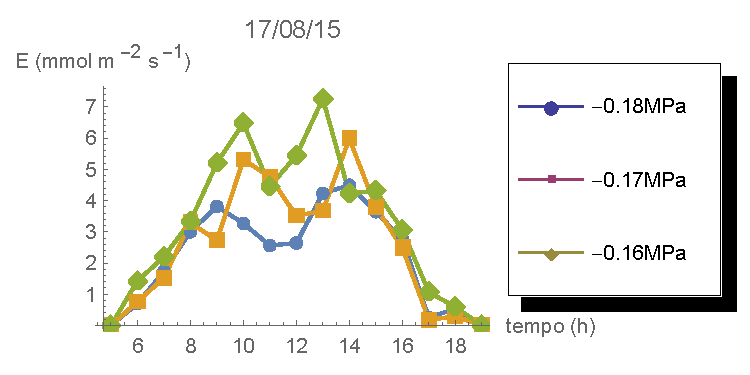
\includegraphics[width=.49\linewidth]{assets/cana/g1_20150817}}
			\subfloat[PAR]{\label{fig:PAR}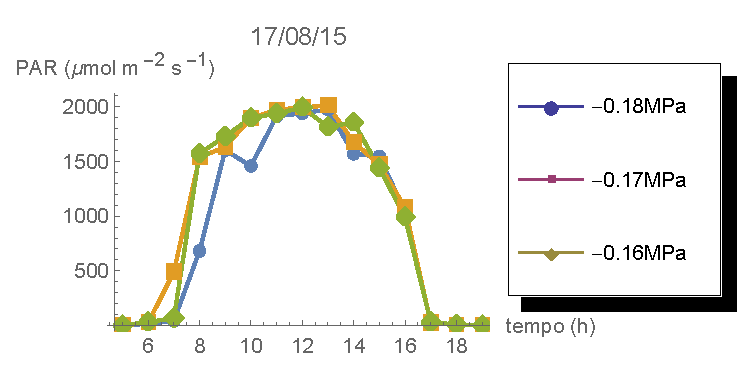
\includegraphics[width=.49\linewidth]{assets/cana/g2_20150817}}\\
			\subfloat[DPV]{\label{fig:DPV}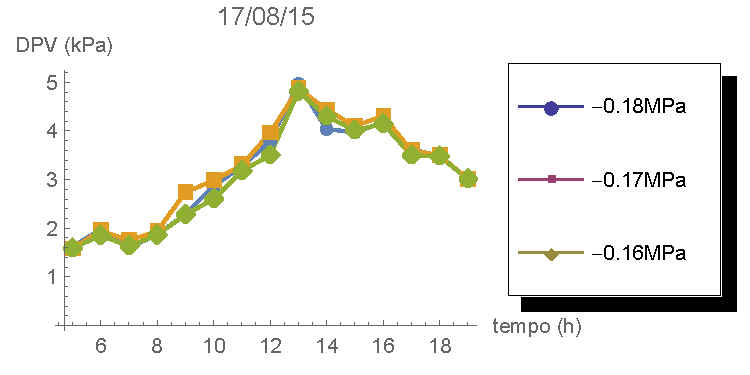
\includegraphics[width=.49\linewidth]{assets/cana/g3_20150817}}
			\subfloat[Transpiração/PAR]{\label{fig:Transpiração/PAR}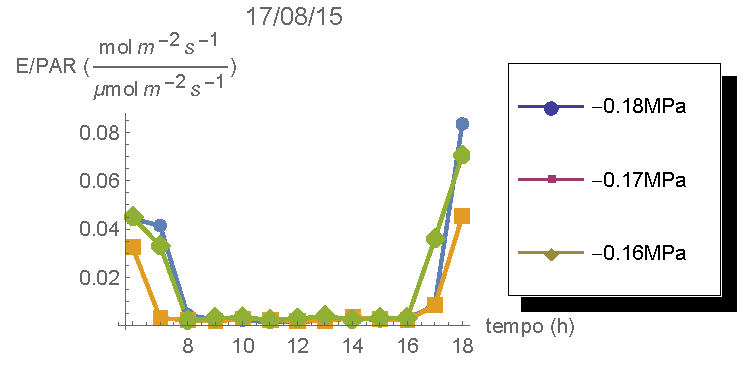
\includegraphics[width=.49\linewidth]{assets/cana/g4_20150817}}\\
			\subfloat[Transpiração/DPV]{\label{fig:Transpiração/DPV}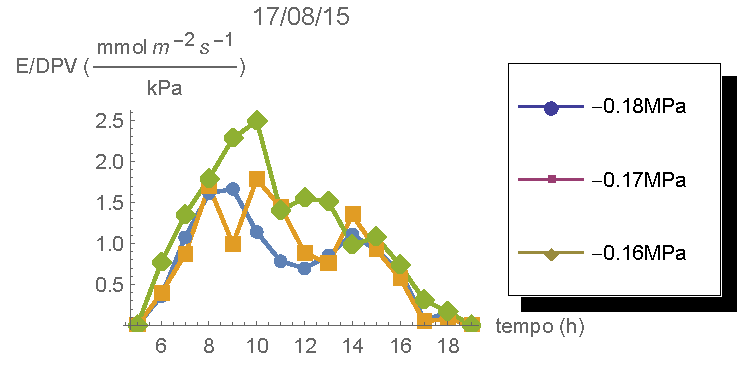
\includegraphics[width=.49\linewidth]{assets/cana/g5_20150817}}
			\caption{Cana de açúcar - 17/08/2015}
			\label{fig:g120150817}
		\end{figure}
		\begin{figure}[H]
			\centering
			\subfloat[Transpiração]{\label{fig:Transpiração}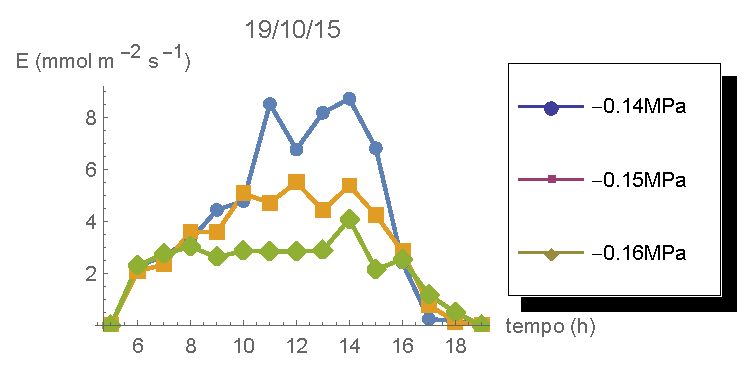
\includegraphics[width=.49\linewidth]{assets/cana/g1_20151019}}
			\subfloat[PAR]{\label{fig:PAR}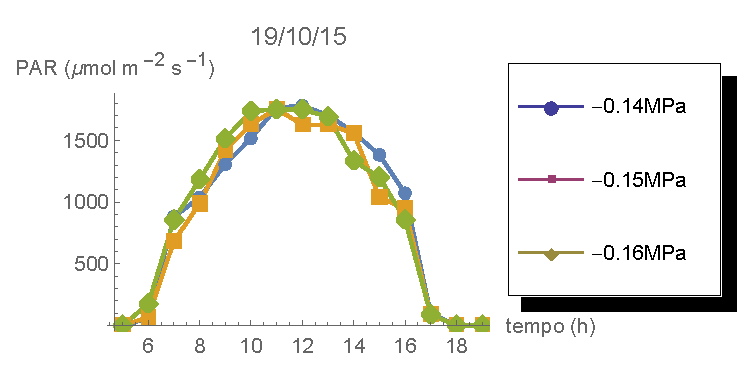
\includegraphics[width=.49\linewidth]{assets/cana/g2_20151019}}\\
			\subfloat[DPV]{\label{fig:DPV}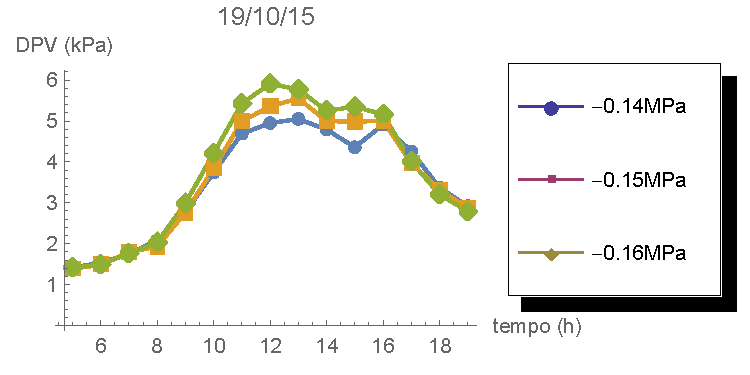
\includegraphics[width=.49\linewidth]{assets/cana/g3_20151019}}
			\subfloat[Transpiração/PAR]{\label{fig:Transpiração/PAR}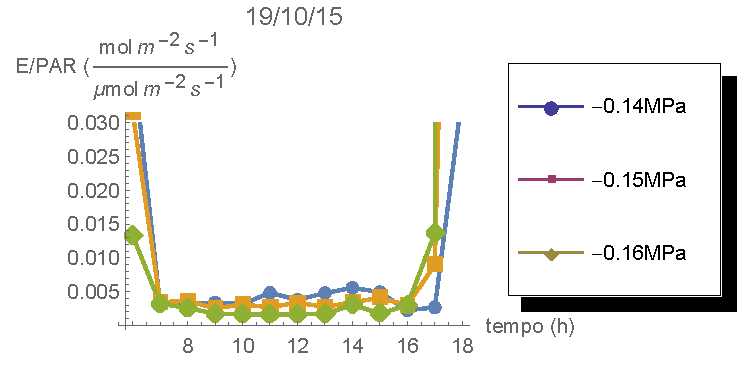
\includegraphics[width=.49\linewidth]{assets/cana/g4_20151019}}\\
			\subfloat[Transpiração/DPV]{\label{fig:Transpiração/DPV}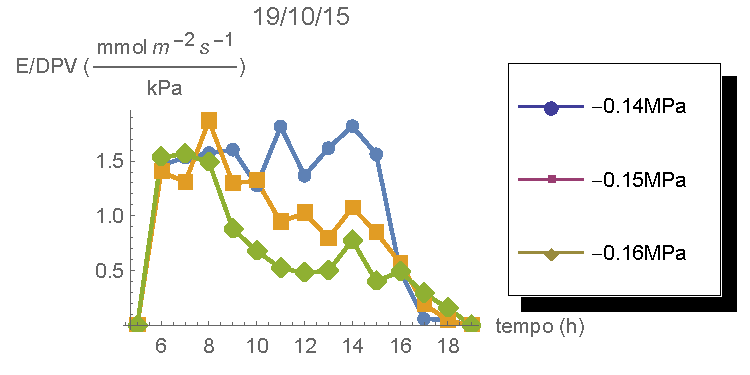
\includegraphics[width=.49\linewidth]{assets/cana/g5_20151019}}
			\caption{Cana de açúcar - 19/10/2015}
			\label{fig:g120151019}
		\end{figure}
	\section{Pata de vaca}
		\begin{figure}[H]
			\centering
			\subfloat[Transpiração]{\label{fig:Transpiração}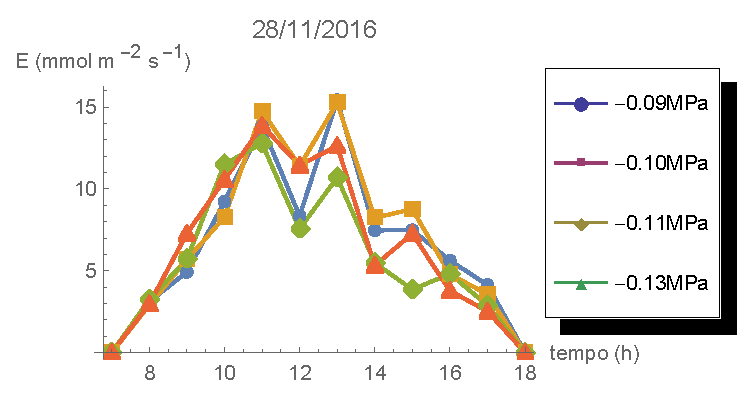
\includegraphics[width=.49\linewidth]{assets/pata/g1_20161128}}
			\subfloat[PAR]{\label{fig:PAR}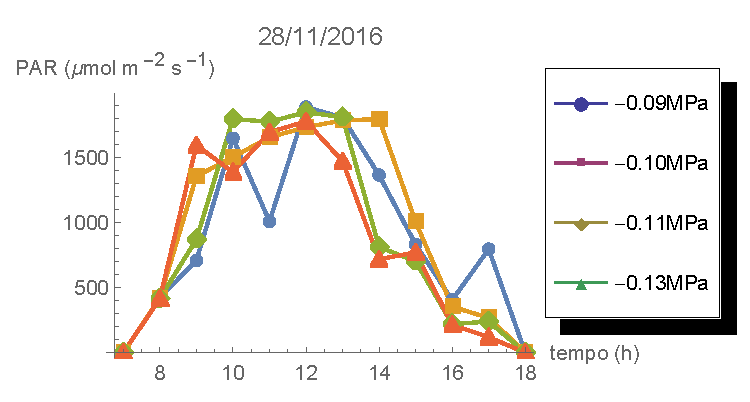
\includegraphics[width=.49\linewidth]{assets/pata/g2_20161128}}\\
			\subfloat[DPV]{\label{fig:DPV}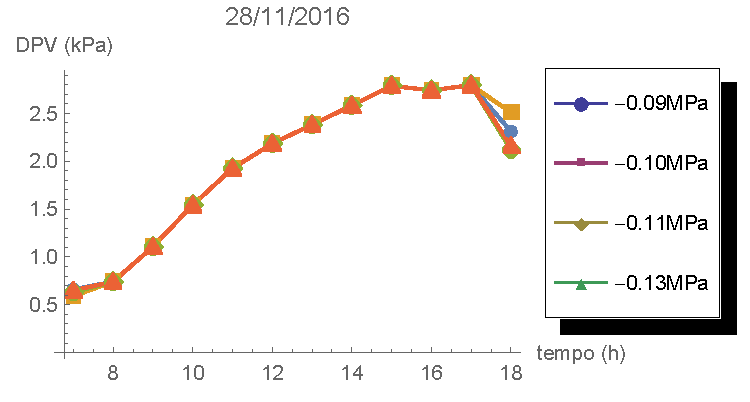
\includegraphics[width=.49\linewidth]{assets/pata/g3_20161128}}
			\subfloat[Transpiração/PAR]{\label{fig:Transpiração/PAR}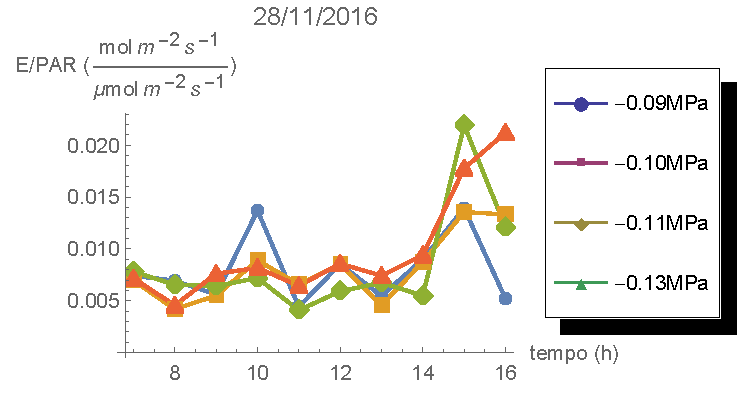
\includegraphics[width=.49\linewidth]{assets/pata/g4_20161128}}\\
			\subfloat[Transpiração/DPV]{\label{fig:Transpiração/DPV}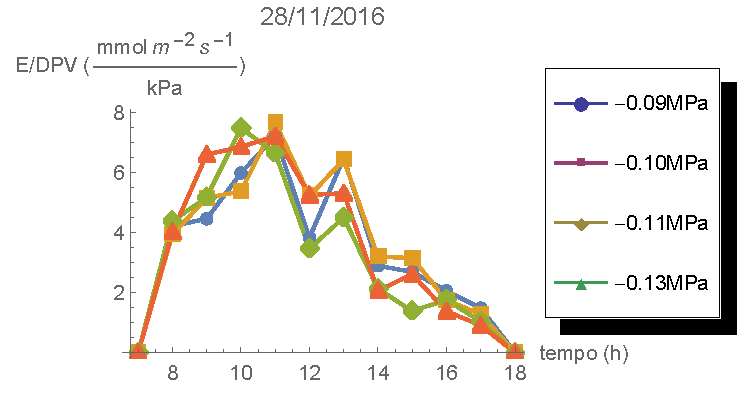
\includegraphics[width=.49\linewidth]{assets/pata/g5_20161128}}
			\caption{Pata de Vaca - 28/11/2016}
			\label{fig:g120161128}
		\end{figure}
	\section{Myrtaceae}
		\begin{figure}[H]
			\centering
			\subfloat[Transpiração]{\label{fig:Transpiração}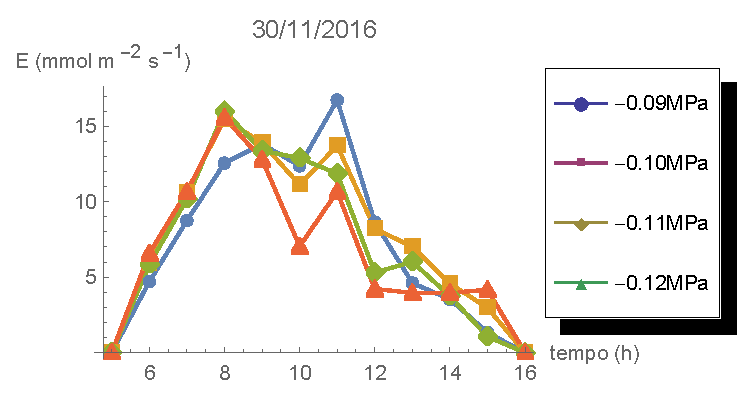
\includegraphics[width=.49\linewidth]{assets/myrtaceae/g1_20161130}}
			\subfloat[PAR]{\label{fig:PAR}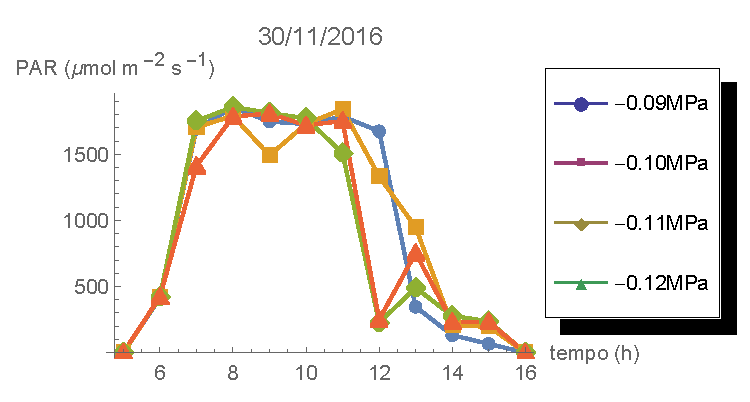
\includegraphics[width=.49\linewidth]{assets/myrtaceae/g2_20161130}}\\
			\subfloat[DPV]{\label{fig:DPV}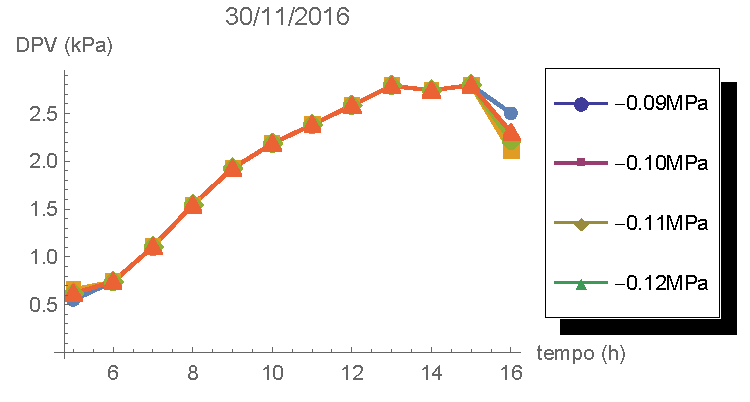
\includegraphics[width=.49\linewidth]{assets/myrtaceae/g3_20161130}}
			\subfloat[Transpiração/PAR]{\label{fig:Transpiração/PAR}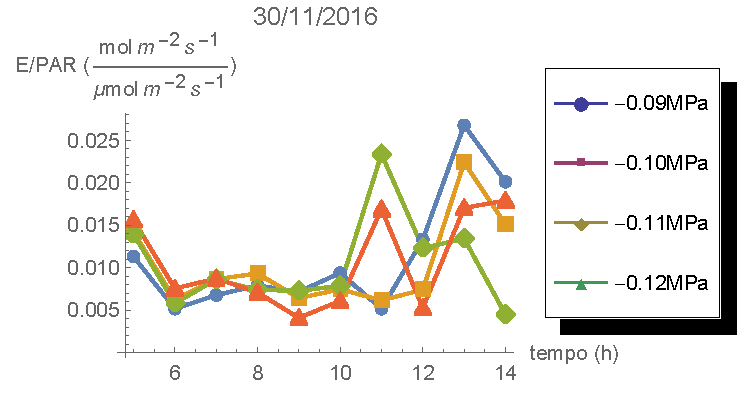
\includegraphics[width=.49\linewidth]{assets/myrtaceae/g4_20161130}}\\
			\subfloat[Transpiração/DPV]{\label{fig:Transpiração/DPV}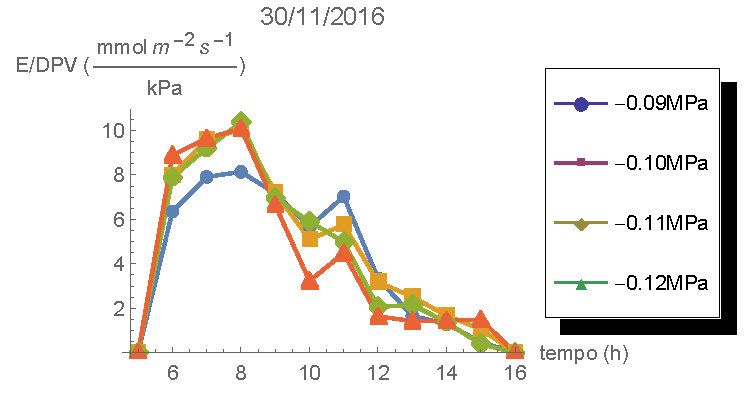
\includegraphics[width=.49\linewidth]{assets/myrtaceae/g5_20161130}}
			\caption{Myrtaceae - 30/11/2016}
			\label{fig:g120161130}
		\end{figure}
	\section{Grumixama}
		\begin{figure}[H]
			\centering
			\subfloat[Transpiração]{\label{fig:Transpiração}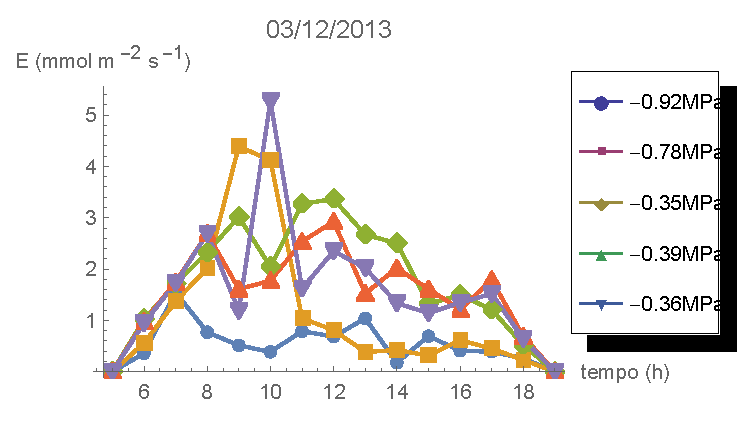
\includegraphics[width=.49\linewidth]{assets/grumixama/g1_20131203}}
			\subfloat[PAR]{\label{fig:PAR}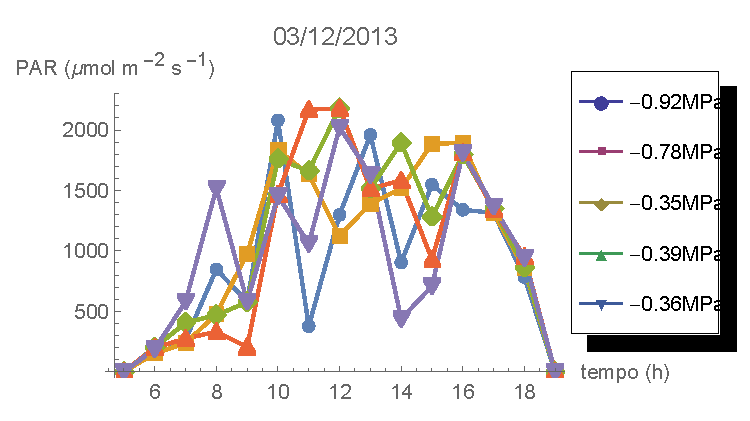
\includegraphics[width=.49\linewidth]{assets/grumixama/g2_20131203}}\\
			\subfloat[DPV]{\label{fig:DPV}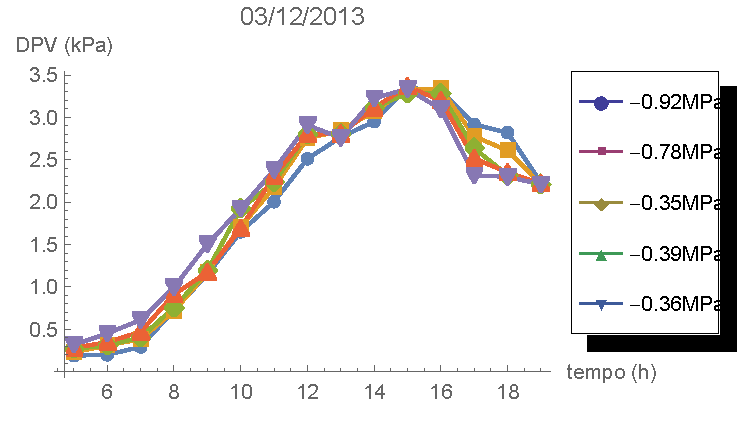
\includegraphics[width=.49\linewidth]{assets/grumixama/g3_20131203}}
			\subfloat[Transpiração/PAR]{\label{fig:Transpiração/PAR}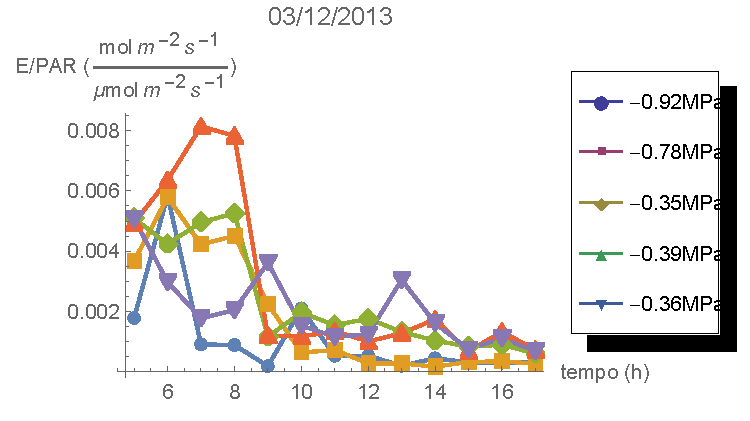
\includegraphics[width=.49\linewidth]{assets/grumixama/g4_20131203}}\\
			\subfloat[Transpiração/DPV]{\label{fig:Transpiração/DPV}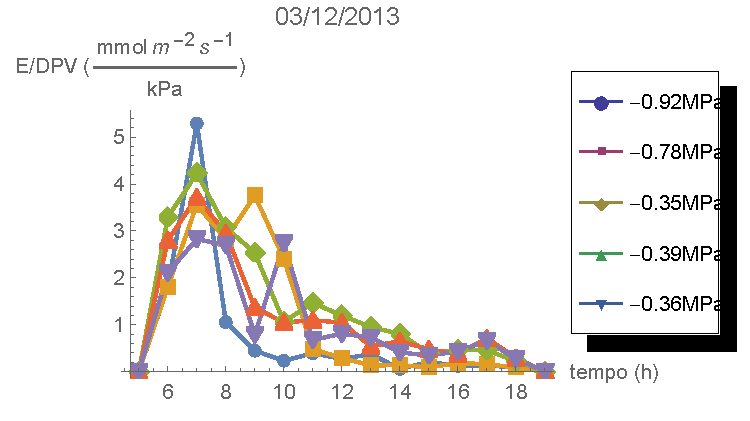
\includegraphics[width=.49\linewidth]{assets/grumixama/g5_20131203}}
			\caption{Grumixama - 03/12/2013}
			\label{fig:g120131203}
		\end{figure}
	\section{Eucalipto}
		\begin{figure}[H]
			\centering
			\subfloat[Transpiração]{\label{fig:Transpiração}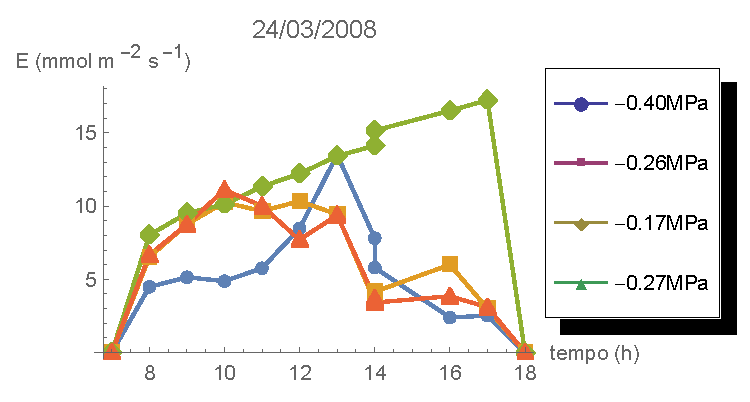
\includegraphics[width=.49\linewidth]{assets/eucalipto/g1_20080324}}
			\subfloat[PAR]{\label{fig:PAR}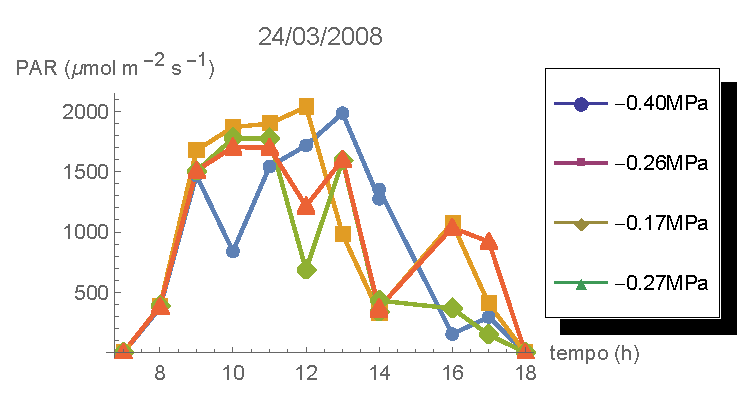
\includegraphics[width=.49\linewidth]{assets/eucalipto/g2_20080324}}\\
			\subfloat[DPV]{\label{fig:DPV}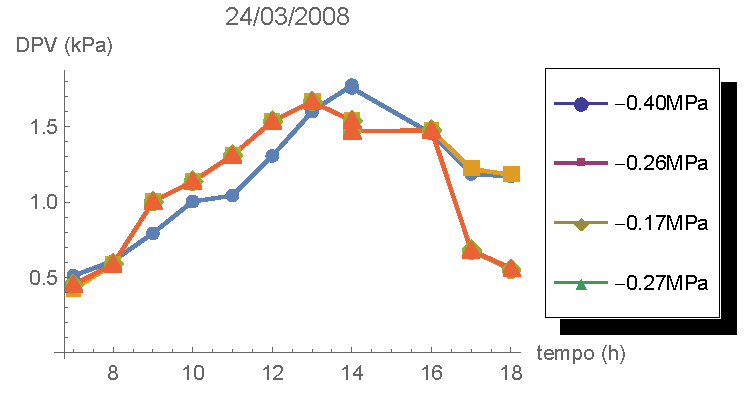
\includegraphics[width=.49\linewidth]{assets/eucalipto/g3_20080324}}
			\subfloat[Transpiração/PAR]{\label{fig:Transpiração/PAR}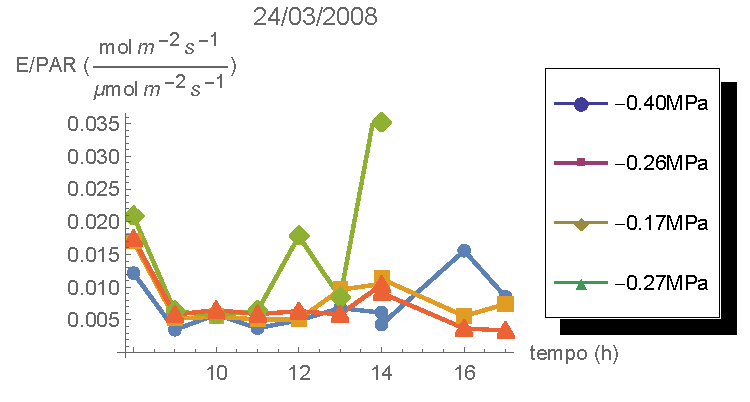
\includegraphics[width=.49\linewidth]{assets/eucalipto/g4_20080324}}\\
			\subfloat[Transpiração/DPV]{\label{fig:Transpiração/DPV}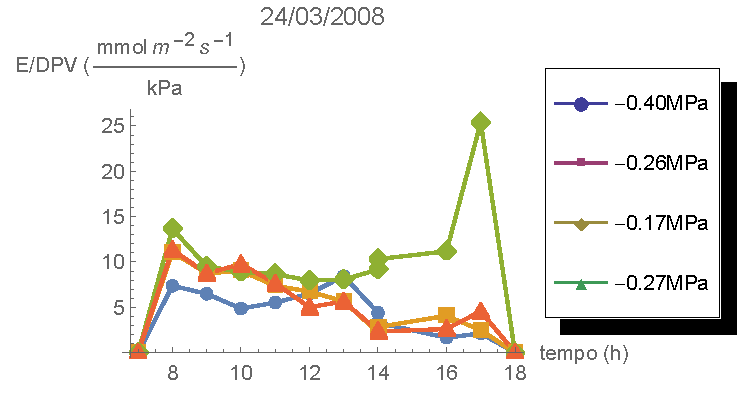
\includegraphics[width=.49\linewidth]{assets/eucalipto/g5_20080324}}
			\caption{Eucalipto - 24/03/2008}
			\label{fig:g120080324}
		\end{figure}
		\begin{figure}[H]
			\centering
			\subfloat[Transpiração]{\label{fig:Transpiração}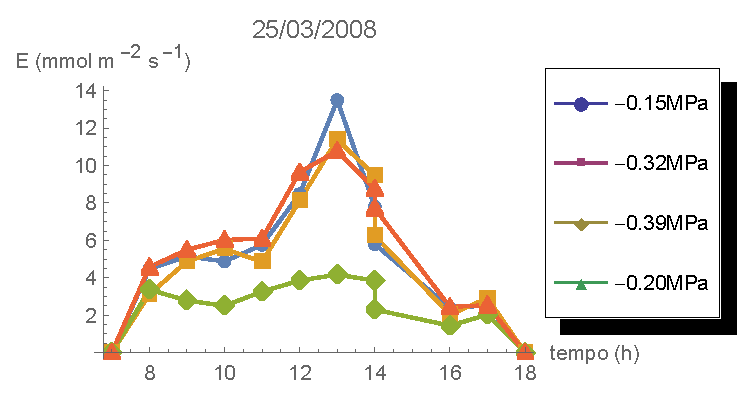
\includegraphics[width=.49\linewidth]{assets/eucalipto/g1_20080325}}
			\subfloat[PAR]{\label{fig:PAR}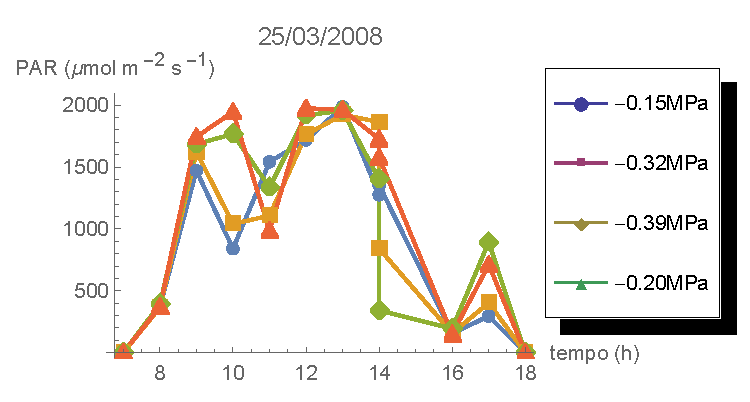
\includegraphics[width=.49\linewidth]{assets/eucalipto/g2_20080325}}\\
			\subfloat[DPV]{\label{fig:DPV}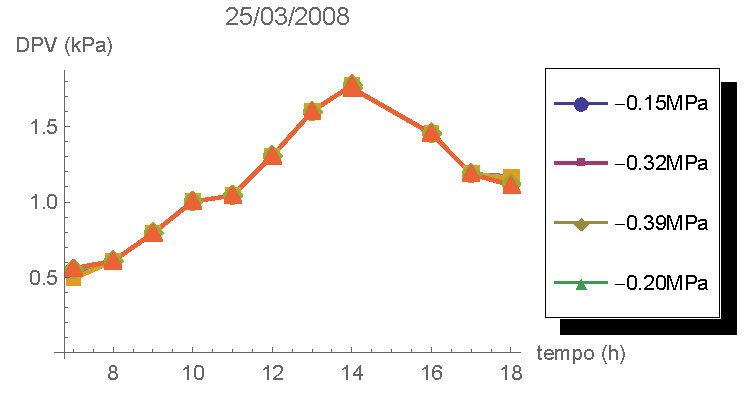
\includegraphics[width=.49\linewidth]{assets/eucalipto/g3_20080325}}
			\subfloat[Transpiração/PAR]{\label{fig:Transpiração/PAR}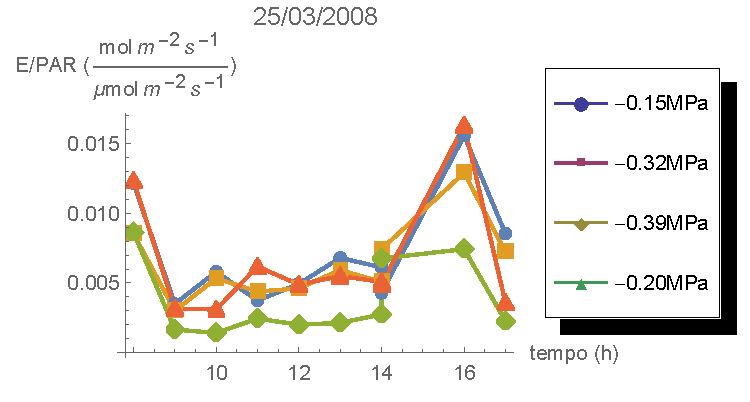
\includegraphics[width=.49\linewidth]{assets/eucalipto/g4_20080325}}\\
			\subfloat[Transpiração/DPV]{\label{fig:Transpiração/DPV}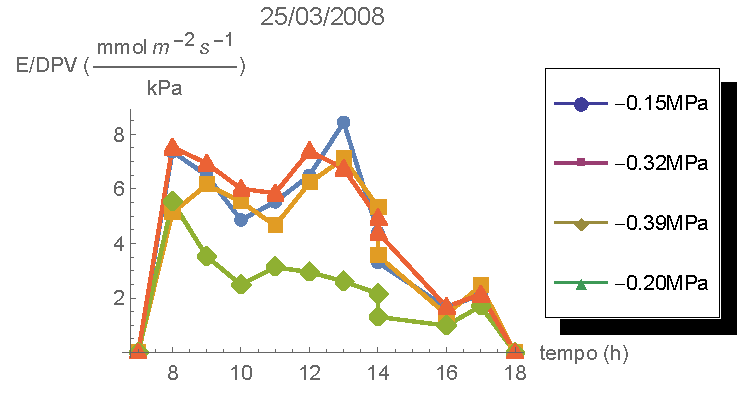
\includegraphics[width=.49\linewidth]{assets/eucalipto/g5_20080325}}
			\caption{Eucalipto - 25/03/2008}
			\label{fig:g120080325}
		\end{figure}
		\begin{figure}[H]
			\centering
			\subfloat[Transpiração]{\label{fig:Transpiração}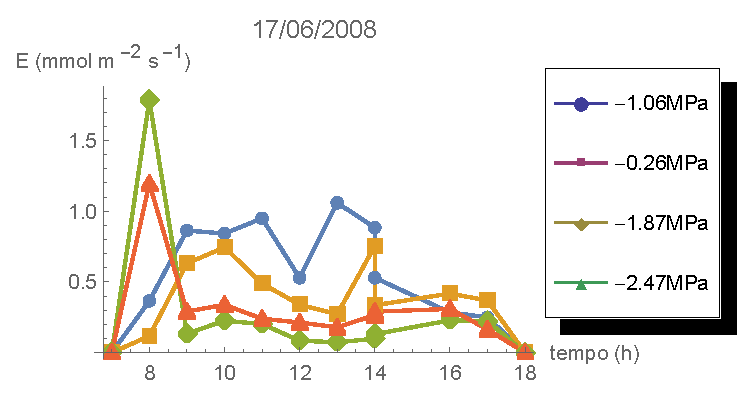
\includegraphics[width=.49\linewidth]{assets/eucalipto/g1_20080617}}
			\subfloat[PAR]{\label{fig:PAR}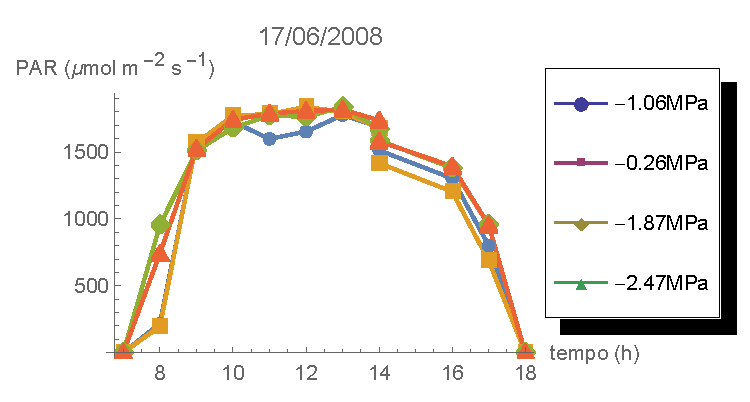
\includegraphics[width=.49\linewidth]{assets/eucalipto/g2_20080617}}\\
			\subfloat[DPV]{\label{fig:DPV}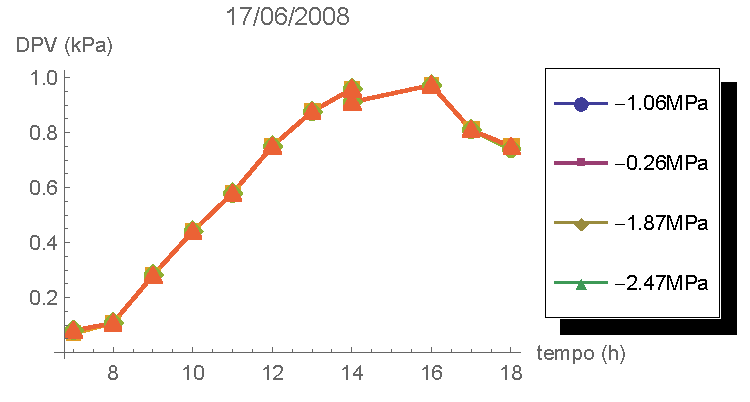
\includegraphics[width=.49\linewidth]{assets/eucalipto/g3_20080617}}
			\subfloat[Transpiração/PAR]{\label{fig:Transpiração/PAR}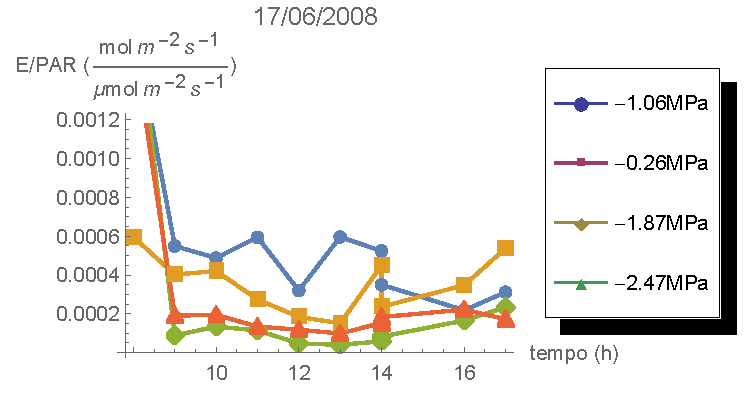
\includegraphics[width=.49\linewidth]{assets/eucalipto/g4_20080617}}\\
			\subfloat[Transpiração/DPV]{\label{fig:Transpiração/DPV}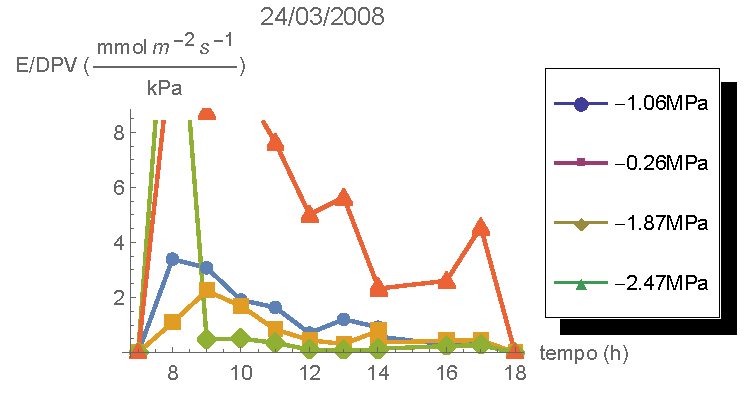
\includegraphics[width=.49\linewidth]{assets/eucalipto/g5_20080617}}
			\caption{Eucalipto - 17/06/2008}
			\label{fig:g120080617}
		\end{figure}
		\begin{figure}[H]
			\centering
			\subfloat[Transpiração]{\label{fig:Transpiração}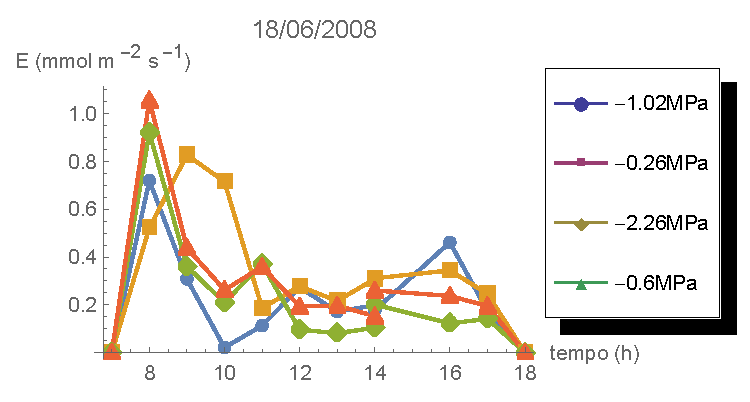
\includegraphics[width=.49\linewidth]{assets/eucalipto/g1_20080618}}
			\subfloat[PAR]{\label{fig:PAR}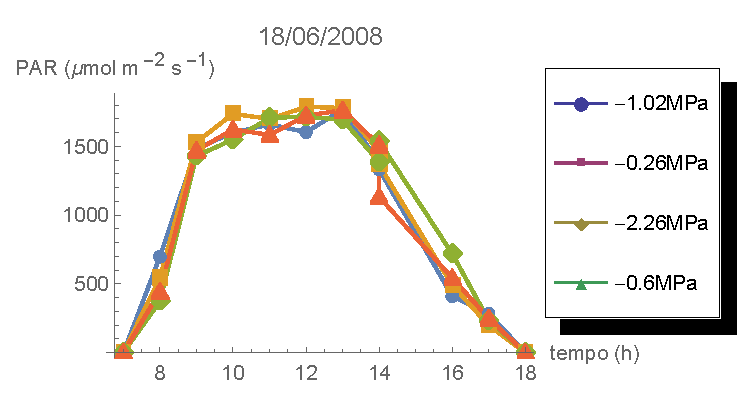
\includegraphics[width=.49\linewidth]{assets/eucalipto/g2_20080618}}\\
			\subfloat[DPV]{\label{fig:DPV}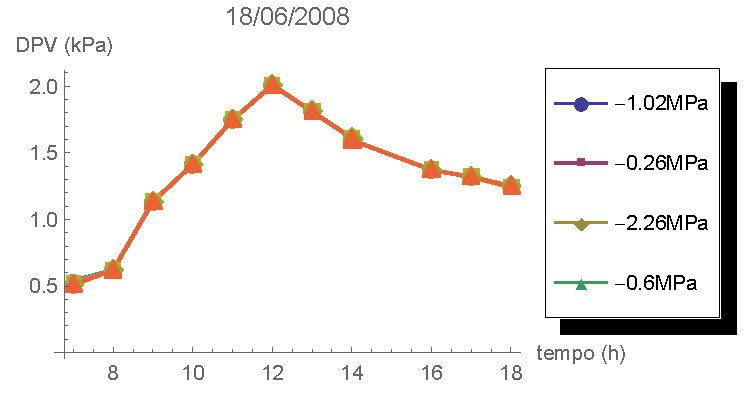
\includegraphics[width=.49\linewidth]{assets/eucalipto/g3_20080618}}
			\subfloat[Transpiração/PAR]{\label{fig:Transpiração/PAR}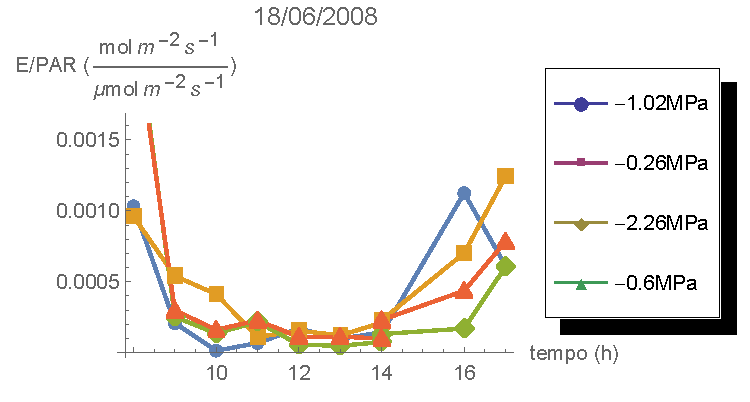
\includegraphics[width=.49\linewidth]{assets/eucalipto/g4_20080618}}\\
			\subfloat[Transpiração/DPV]{\label{fig:Transpiração/DPV}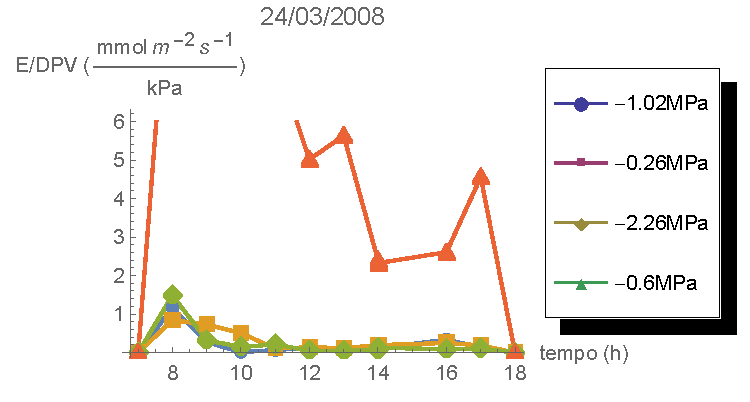
\includegraphics[width=.49\linewidth]{assets/eucalipto/g5_20080618}}
			\caption{Eucalipto - 18/06/2008}
			\label{fig:g120080618}
		\end{figure}
\end{document}